\section{Preliminaries}\label{sec:prelims}

We begin by introducing some necessary observations, definitions, and terminology
which will be of use later.  
\subsection{Spherical Geometry}

In this section, we present some basic results about spherical geometry with the goal of proving Girard's Theorem, which states that the area of a triangle on the unit sphere is the sum of its interior angles minus $\pi$.  Readers familiar with this result should feel free to skip ahead.



We use $\R^2$ to denote the 
Euclidean plane with the usual way of measuring distances, 
$$d(x,y) = \sqrt{(x-y)^2};$$
similarly, $\R^3$ denotes Euclidean 3-space.  We use $\mbb{S}^2$ to denote the \textit{unit 2-sphere}, which can be 
thought of as the set of points in $\R^3$ at Euclidean distance one from the origin.  
 
In this paper, we only consider the sphere and the plane, and leave the consideration of other surfaces, measures, and metrics to future work.







\begin{definition}
{On the sphere, a \textbf{great circle} is the intersection of the sphere with a plane passing through the origin.} These are the circles on the sphere with radius equal to that of the sphere.  See \Cref{fig:sphereline} for an illustration.
\end{definition}

\begin{definition}

Lines in the plane and great circles on the sphere are called \textbf{geodesics}.  A \textbf{geodesic segment} is a line segment in the plane and an arc of a great circle on the sphere.
	
\end{definition}  



{The idea of {geodesics} generalizes the notion of \enquote*{straight lines} in the plane to other settings.} One critical difference is that in the plane, there is a unique line passing through any two distinct points and a unique line segment joining them.  On the sphere, there will typically be a unique great circle and \textit{two} geodesic segments through a pair of points, with the exception of one case.


\begin{definition}
	A \textbf{triangle} in the plane or the sphere is defined by three distinct points and the shortest geodesics connecting each pair of points.
\end{definition}






{
\ifsmallfigs
\else
\begin{figure}[htb]
	\centering
	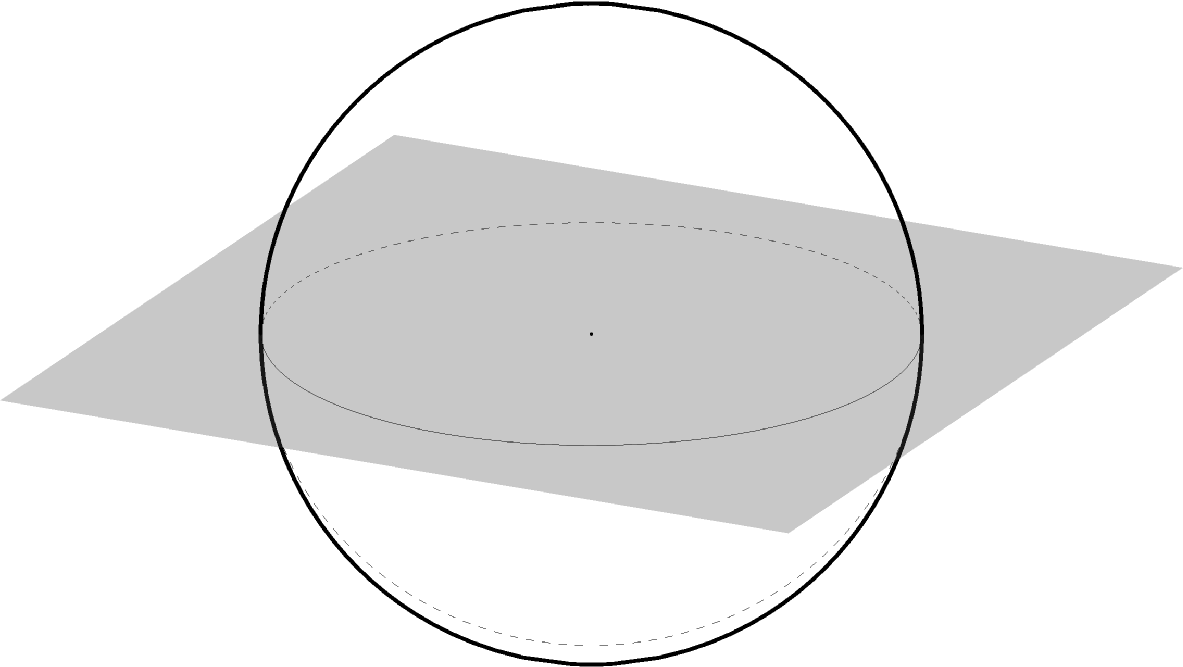
\includegraphics[width=.5\textwidth]{figs/sph-1pl.pdf}
	\caption{A great circle on the sphere with its identifying plane.}
	\label{fig:sphereline}
\end{figure}
\fi
}



\begin{observation}
	Given any two points $p$ and $q$ on the sphere which are not antipodal, meaning that our points aren't of the form $p=(x,y,z)$ and $q=(-x,-y,-z)$, there is a unique great circle through $p$ and $q$ and therefore two geodesic segments joining them. 
\end{observation}
\mute{
\begin{proof}
	To see this, consider the characterization of great circles as the intersections of the surface of the sphere with planes through the center of the sphere.  Since $p$ and $q$ are not antipodes, they are not both collinear with $(0,0,0)$ and so these three points uniquely determine a plane.  This plane intersects the sphere along a great circle which contains $p$ and $q$.
\end{proof}
}
If $p$ and $q$ \textit{are} antipodal, then any great circle containing one must contain the other as well, so there are infinitely many such great circles. For any two non-antipodal points on the sphere, one of the geodesic segments will be shorter than the other.  {This shorter geodesic segment is the shortest path between the points and its length is the metric distance between $p$ and $q$}.

\ifsmallfigs
\begin{figure}
	\centering
	\begin{minipage}{.5\textwidth}
		\centering
	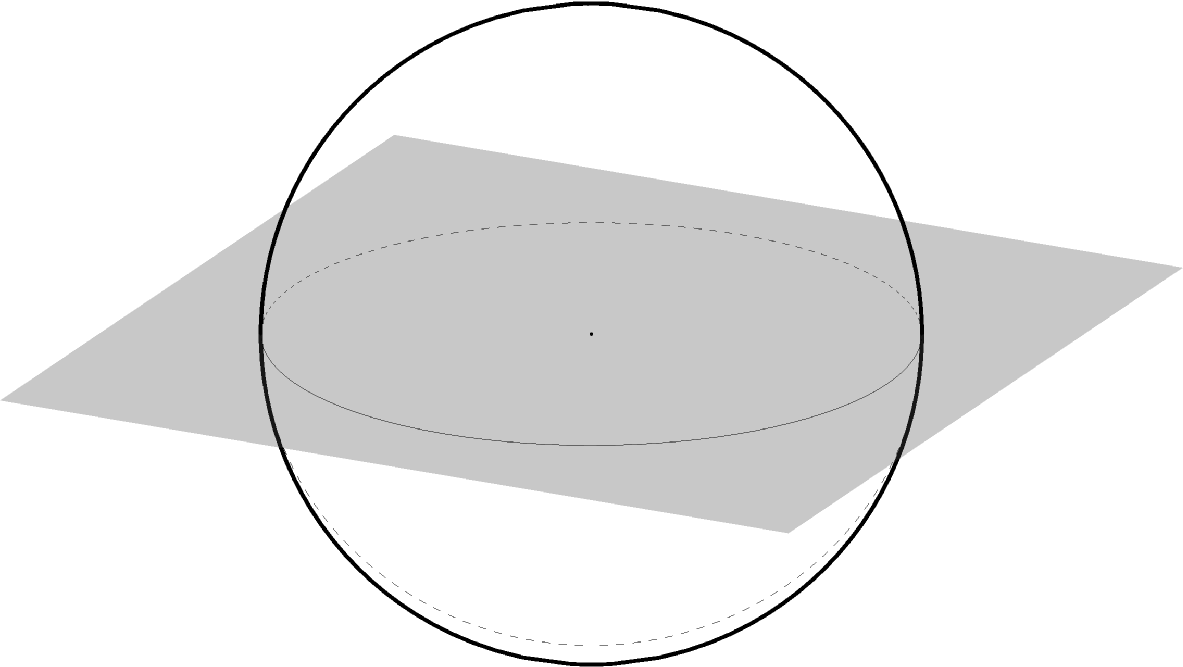
\includegraphics[height=.58\linewidth]{figs/sph-1pl.pdf}
		\captionof{figure}{A great circle on the sphere with its plane.}
		\label{fig:test1}
	\end{minipage}%
	\begin{minipage}{.5\textwidth}
		\centering
	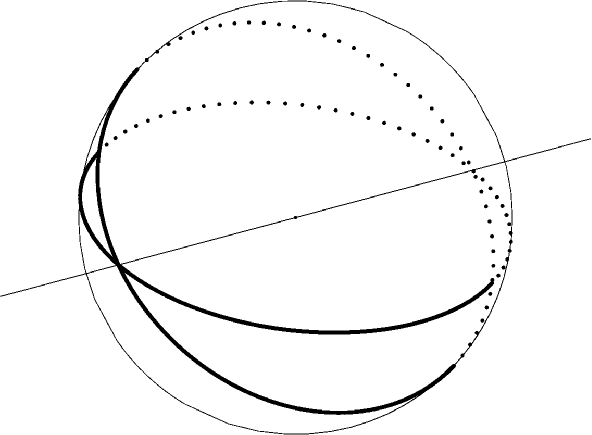
\includegraphics[height=.58\linewidth]{figs/2gc.pdf}
		\captionof{figure}{Two great circles meet at antipodal points.}
	\label{fig:sphereline}
	\end{minipage}
\end{figure}
\fi


\ifsmallfigs
\else
\begin{figure}[htb]
	\centering
	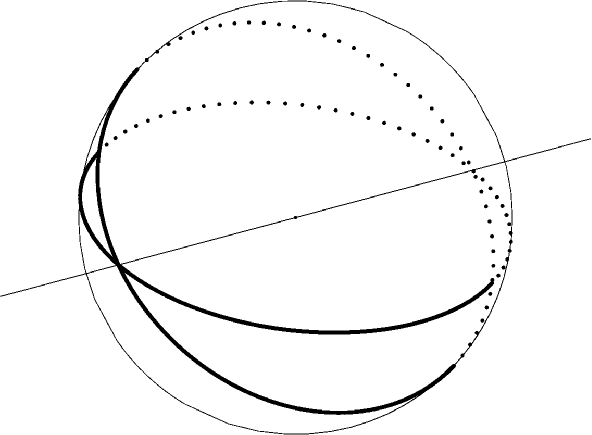
\includegraphics[width=.35\textwidth]{figs/2gc.pdf}
	\caption{Two great circles meet at antipodal points.}
	\label{fig:2gc}
\end{figure}
\fi


We now have enough terminology to show a very important fact about spherical geometry.  This  observation is one of the salient features which distinguishes it from the more familiar planar geometry.


\begin{claim}
	Any pair of distinct great circles on the sphere intersect exactly twice, and the points of intersection are antipodes.
\end{claim}
\mute{
\begin{proof}
	Any two distinct planes determine two distinct great circles, and these planes intersect along a line in $\R^3$ which passes through $(0,0,0)$ and therefore meets the sphere itself at exactly two points, which must be antipodes.
\end{proof}
}



Why is this weird? In the plane, it is always the case that any pair of distinct lines intersects exactly once or never, in which case we call them \textit{parallel}. Since distinct great circles on the sphere intersect exactly twice, there is no such thing as \enquote*{parallel lines} on the sphere, and we have to be careful about discussing `the' intersection of two great circles since they do not meet at a unique point.  Furthermore, it is not the case that there is a unique segment of a great circle connecting any two points; there are two, but unless our two points are antipodes, one of the two segments will be shorter. 



\mute{We will use this distinction to derive a result which we will use critically in the main theorems of this paper, namely\\

\noindent\textbf{\Cref{lem:sphtri}.} [Girard's Theorem]
\emph{The sum of the interior angles of a spherical triangle is strictly greater than $\pi$.  More specifically, the sum of the interior angles is equal to $\pi$ plus the area of the triangle.}\\}

Another difference between spherical and planar geometry appears when computing the angles of triangles. In the planar setting, the sum of the interior angles of a triangle is always $\pi$, regardless of its area. However, in the spherical case we can construct a triangle with three right angles. The north pole and two points on the equator, one a quarter of the way around the sphere from the other, form such a triangle.  Its area is one eighth of the whole sphere, or $\tfrac{\pi}{2}$, which is, not coincidentally, equal to $\tfrac{\pi}{2}+\tfrac{\pi}{2}+\tfrac{\pi}{2} - \pi$. Girard's theorem, which we will prove below, connects the total angle to the area of a spherical triangle.


In order to  show Girard's Theorem, we need some way to translate between \textit{angles} and \textit{area}.  To do that, we'll use a shape which doesn't even exist in the plane: the \textit{diangle} or \textit{lune}.    We know that two great circles intersect at two antipodal points, and we can also see that they cut the surface of the sphere into four regions.  Consider one of these regions.  Its boundary is a pair of great circle segments which connect antipodal points and meet at some angle $\theta\leq \pi$ at both of these points.   

Using that the surface area of a unit sphere is $4\pi$, computing the area of a lune with angle $\theta$ is straightforward.


\begin{figure}[htb]
	\centering
	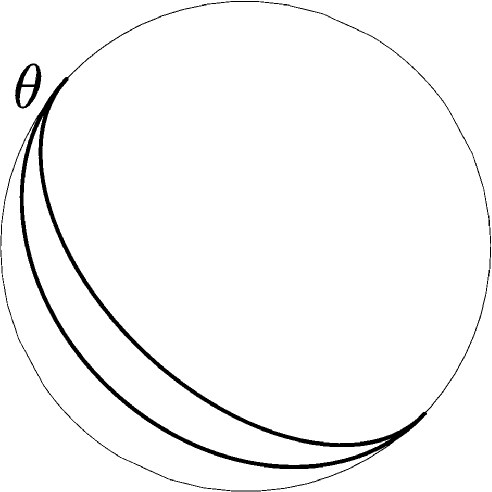
\includegraphics[width=.35\textwidth]{figs/lune.pdf}
	\caption{A lune corresponding to an angle $\theta$. }
	\label{fig:lune}
\end{figure}
		\begin{figure}[htb]
	\centering
	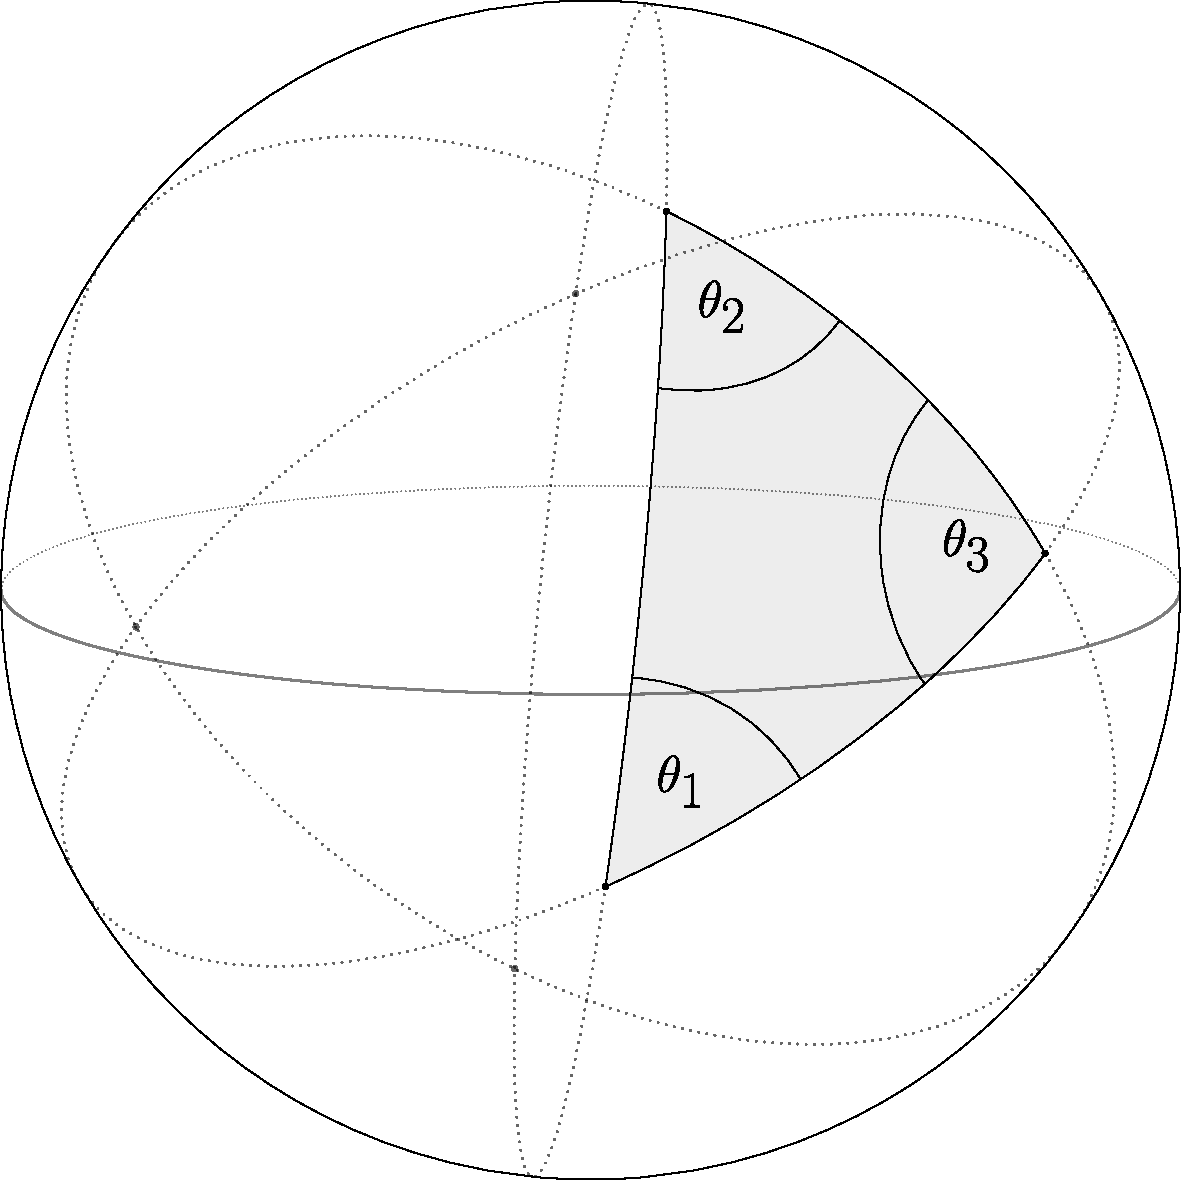
\includegraphics[width=.35\textwidth]{figs/trilune.pdf}
	\caption{A spherical triangle and the antipodal triangle define six lunes.}
	\label{fig:trilune}
\end{figure}

\begin{claim}
	Consider a lune whose boundary segments meet at angle $\theta$.  Then the area of this lune is $2\theta$.
\end{claim}

Now that we have a tool that lets us relate angles and areas, we can prove Girard's Theorem.










\begin{lemma}(Girard's Theorem)\label{lem:sphtri}
	
	The sum of the interior angles of a spherical triangle is strictly greater than $\pi$.  More specifically, the sum of the interior angles is equal to $\pi$ plus the area of the triangle.
\end{lemma}

\begin{proof}
	Consider a triangle $T$ on the sphere with angles $\theta_1$, $\theta_2$, and $\theta_3$.  Let $\mathrm{area}(T)$ denote the area of this triangle. If we extend the sides of the triangle to their entire great circles, each pair intersects at the vertices of $T$ as well as the three points antipodal to the vertices of $T$, and at the same angles at antipodal points.  This second triangle is congruent to $T$, so its area is also $\mathrm{area}(T)$.  Each pair of great circles cuts the sphere into four lunes, one which contains $T$, one which contains the antipodal triangle, and two which do not contain either triangle.  We are interested in the three pairs of lunes which do contain the triangles.  We will label these lunes by their angles, so we have a lune $L(\theta_1)$ and its antipodal lune $L'(\theta_1)$, and we can similarly define $L(\theta_2)$, $L'(\theta_2)$, $L(\theta_3)$, and $L'(\theta_3)$.
	
	

	
	
	We have six lunes.  In total, they cover the sphere, but share some overlap.  If we remove $T$ from two of the three which contain it and the antipodal triangle from two of the three which contain it, then we have six non-overlapping regions which cover the sphere, so the area of the sphere must be equal to the sum of the areas of these six regions.  \mute{We can write
	
	\begin{align*}
	4\pi &= \mathrm{area}(L(\theta_1)) + \mathrm{area}(L'(\theta_1)) \\
	&+  (\mathrm{area}(L(\theta_2)) - \mathrm{area}(T)) + (\mathrm{area}(L'(\theta_2)) - \mathrm{area}(T)) \\
	&+ (\mathrm{area}(L(\theta_3)) - \mathrm{area}(T))	 + (\mathrm{area}(L'(\theta_3)) - \mathrm{area}(T)).
	\end{align*}
}
	
	

	
	By the earlier claim, we know that the areas of the lunes are twice their angles, so we can write this as
	
	\ifarxiv
	\begin{align*}
	4\pi &= 2\theta_1 + 2\theta_1 
	+  (2\theta_2 - \mathrm{area}(T)) + (2\theta_2-\mathrm{area}(T))
	+ (2\theta_3 - \mathrm{area}(T))	 + (2\theta_3 - \mathrm{area}(T))
	\end{align*}
	\else
\begin{align*}
4\pi &= 2\theta_1 + 2\theta_1 
+  (2\theta_2 - \mathrm{area}(T)) + (2\theta_2-\mathrm{area}(T))\\
&\phantom{2\pi} + (2\theta_3 - \mathrm{area}(T))	 + (2\theta_3 - \mathrm{area}(T))
\end{align*}	
	\fi
	and rearrange to get
	
	
	\begin{align*}
	\theta_1+\theta_2+\theta_3 = \pi + \mathrm{area}(T),
	\end{align*}
	
	which is exactly the statement we wanted to show.
\end{proof}

We will need one more fact about spherical triangles before we conclude this section.  It follows immediately from the Spherical Law of Cosines.

\begin{fact}
	An equilateral triangle is equiangular, and vice versa, where \textit{equilateral} means that the three sides have equal length and \textit{equiangular} means that the three angles all have the same measure.
\end{fact}


\mute{
\begin{proof}
	To see this, first suppose that we have a triangle with vertices $a$, $b$, and $c$ and suppose that the length of the side $ab$ is equal to that of $bc$, and let $m$ be the midpoint of the segment $bc$.  Consider the segment $am$. This splits the triangle $abc$ into two triangles $amb$ and $amc$.  These three triangles have the same side lengths and are therefore congruent.  By this congruence, the angle opposite vertex $a$ is equal to the angle opposite vertex $c$.  To show that either of these is also equal to the angle opposite vertex $b$, take $m$ to be the midpoint of segment $ac$.
	
	To see the converse, suppose that the angles at vertices $b$ and $c$ are equal.  Then the triangle $abc$ is congruent to the triangle $acb$ because they both share side $bc$ and the angle at vertex $a$, and the angle at vertex $b$ is equal to that at $c$.\footnote{This is sometimes called the \enquote{side-side-angle} congruence theorem.}  Since the triangles are congruent, the sides $ac$ and $ab$ have equal length.  To show that either of these is also equal to the length of side $bc$, consider angles $a$ and $c$ instead.
\end{proof}

}

An astute reader may notice that this result is also true of planar triangles, and the planar version follows from Propositions I.6 and I.8 in Euclid's \textit{Elements} \cite{elements,se_triangle}.  Since Euclid's proof doesn't rely on the existence of parallel lines, this fact can alternatively be shown using his argument.



\subsection{Some Definitions}

Now that we have the necessary tools of spherical geometry, we will wrap up this section with a battery of definitions. 
We carefully lay these out so
as to align with an intuitive understanding of the concepts and to
appease the astute reader who may be concerned with edge cases,
geometric weirdness, and nonmeasurability. 
Throughout, we implicitly consider all figures on the sphere to be strictly contained in a hemisphere.








\begin{definition}
	A \textbf{region} is a non-empty, open subset $\Omega$ of $\mathbb{S}^2$ or $\R^2$ such that $\Omega$ is bounded and its boundary is piecewise smooth.
\end{definition}

We choose this definition to ensure that the \textit{area} and \textit{perimeter} of the region are well-defined concepts.  This eliminates pathological examples of open sets whose boundaries have non-zero area or edge cases like considering the whole plane a \enquote*{region}.











\begin{definition}
A \textbf{compactness score function} $\mathcal{C}$ is a function from
the set of all regions to the non-negative real numbers or infinity.  We can compare 
the scores of any two regions, and we adopt the convention that 
\textit{more compact} regions have \textit{higher} scores.  That is,
region $A$ is at least as compact as region $B$ if and only if 
$\mathcal{C}(A)\geq    \mathcal{C}(B)$.
\end{definition}

The final major definition we need is that of a \textit{map
projection}.  In reality, the regions we are interested in comparing
sit on the surface of the Earth (i.e. a sphere), but these regions are
often examined after being projected onto a flat sheet of paper or
computer screen, and so have been subject to such a projection.

\begin{definition}
  A \textbf{map projection} $\varphi$ is a 
  diffeomorphism from a region on the sphere to a region of the 
  plane. 
\end{definition}

We choose this definition, and particularly the term \textit{diffeomorphism}, to ensure that $\vphi$ is smooth, its inverse $\vphi^{-1}$ exists and is smooth, and both $\vphi$ and $\vphi^{-1}$ send regions in their domain to regions in their codomain.  Throughout, we use $\vphi$ to denote such a function from a region of the sphere 
to a region of the plane and $\vphi^{-1}$, to denote the inverse which is a function from a region of the plane back to a region of the sphere.


Since the image of a region under a map projection $\varphi$ is also
a region, we can examine the compactness score of that region both 
before and after applying $\varphi$, and this is the heart of the
problem we address in this paper.  We demonstrate, for several
examples of compactness scores $\mathcal{C}$, that the order
induced by $\mathcal{C}$ is different than the order induced by
$\mathcal{C}\circ\varphi$ for \textit{any} choice of map projection
$\varphi$.

\begin{definition}
  We say that a map projection $\vphi$ \textbf{preserves the  
  compactness score ordering} of a score $\mc{C}$ if for any regions 
  $\Omega,\Omega'$ in the domain of $\vphi$, $\mc{C}(\Omega)\ge \mc{C}(\Omega')$ 
  if and only if $\mc{C}(\vphi(\Omega)) \ge \mc{C}(\vphi(\Omega'))$ in the plane.
\end{definition}

   This is a weaker condition than simply preserving the raw compactness scores. 
   If there is some map projection which results in adding $.1$ to the score of each region, the raw scores are certainly not preserved, but the ordering of regions by their scores is. Additionally, $\vphi$ preserves a compactness score ordering 
  if and only if $\vphi^{-1}$ does.



\begin{definition}
  A 
  \textbf{cap} on the sphere  $\mbb{S}^2$ is a region on the sphere
 which can be described as all of the points on the sphere to one side of some plane 
 in $\R^3$.  A cap has a \textit{height}, which is the largest distance between this cutting plane and the cap, and a \textit{radius}, which is the radius of the circle formed by the intersection of the plane and the sphere.  See \Cref{fig:caphr} for an illustration.
\end{definition}


\begin{figure}[h]
  \centering
  %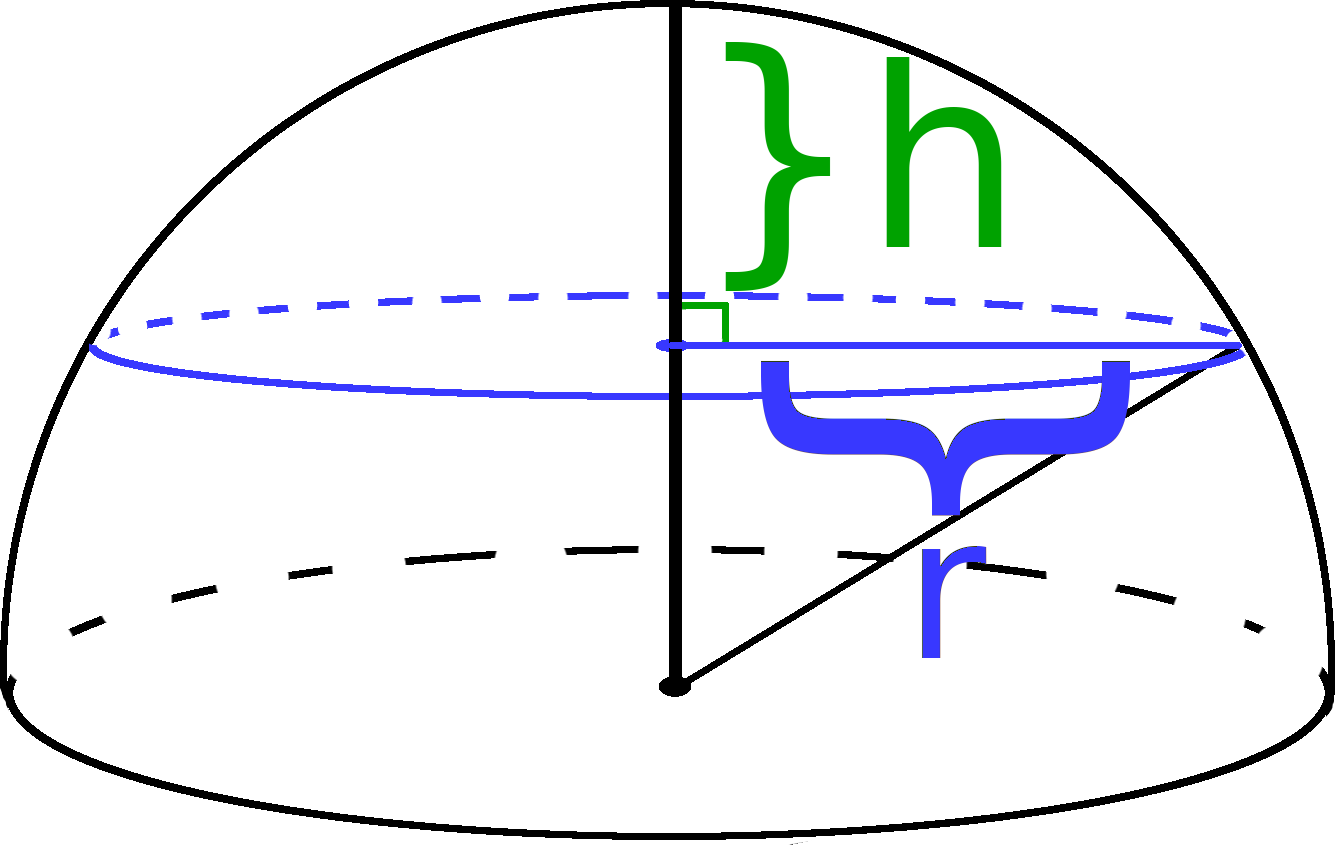
\includegraphics[width=.3\textwidth]{figs/spherecapschema}\\[1.5em]
  \definecolor{qqqqff}{rgb}{0,0,1}

\definecolor{ccqqqq}{rgb}{0.8,0,0}

\definecolor{ududff}{rgb}{0.30196078431372547,0.30196078431372547,1}

\begin{tikzpicture}[line cap=round,line join=round,>=triangle 45,x=1cm,y=1cm]

\clip(-4.493355050909743,-1.2748355780287404) rectangle (4.462150807191927,4.785872976331056);

\draw [shift={(0,0)},line width=3.2pt]  plot[domain=0:3.141592653589793,variable=\t]({1*4*cos(\t r)+0*4*sin(\t r)},{0*4*cos(\t r)+1*4*sin(\t r)});

\draw [shift={(0.0016366799970421299,9.441278259356354)},line width=2pt]  plot[domain=4.286394541961201:5.138764290071874,variable=\t]({1*7.708897306730456*cos(\t r)+0*7.708897306730456*sin(\t r)},{0*7.708897306730456*cos(\t r)+1*7.708897306730456*sin(\t r)});

\draw [shift={(0.019848790872865698,-6.481795867514522)},line width=2pt,dotted]  plot[domain=1.22830273729039:1.9174384984929125,variable=\t]({1*9.441973016351305*cos(\t r)+0*9.441973016351305*sin(\t r)},{0*9.441973016351305*cos(\t r)+1*9.441973016351305*sin(\t r)});

\draw [line width=2pt,color=ccqqqq] (0,2.4033620491027756)-- (0,4);

\draw [line width=2pt,color=qqqqff] (0,2.4033620491027756)-- (3.2001911763834157,2.3997450770024993);

\begin{scriptsize}

\draw [fill=ududff] (0.0016366799970421299,9.441278259356354) circle (2.5pt);

\draw [fill=ududff] (0.019848790872865698,-6.481795867514522) circle (2.5pt);

\draw[color=ccqqqq] (0.26805571312169243,3.3034918797019284) node {\LARGE$h$};

\draw[color=qqqqff] (1.6285727817769453,2.167711482419824) node {\LARGE $r$};

\end{scriptsize}

\end{tikzpicture}
  \caption{ The height $h$ and radius $r$ of a spherical cap. }
  \label{fig:caphr}
\end{figure}





